Leonardo acaba de comprar um laser e decidiu trollar Alberto, um de seus amigos, ao apontar seu laser para ele. Ambos estão na mesma sala, então para que não fique óbvio quem está com o laser, ele decidiu não apontar diretamente, mas através de um espelho. A sala pode ser considerada como um plano cartesiano 2D infinito, em que Leonardo e Alberto são os pontos com coordenadas $(x_L, y_L)$ e $(x_A, y_A)$, respectivamente, e o espelho, que reflete para ambos os lados, é representado por um segmento de reta unindo os pontos $(x_{E1}, y_{E1})$ e $(x_{E2}, y_{E2})$.

\begin{center}
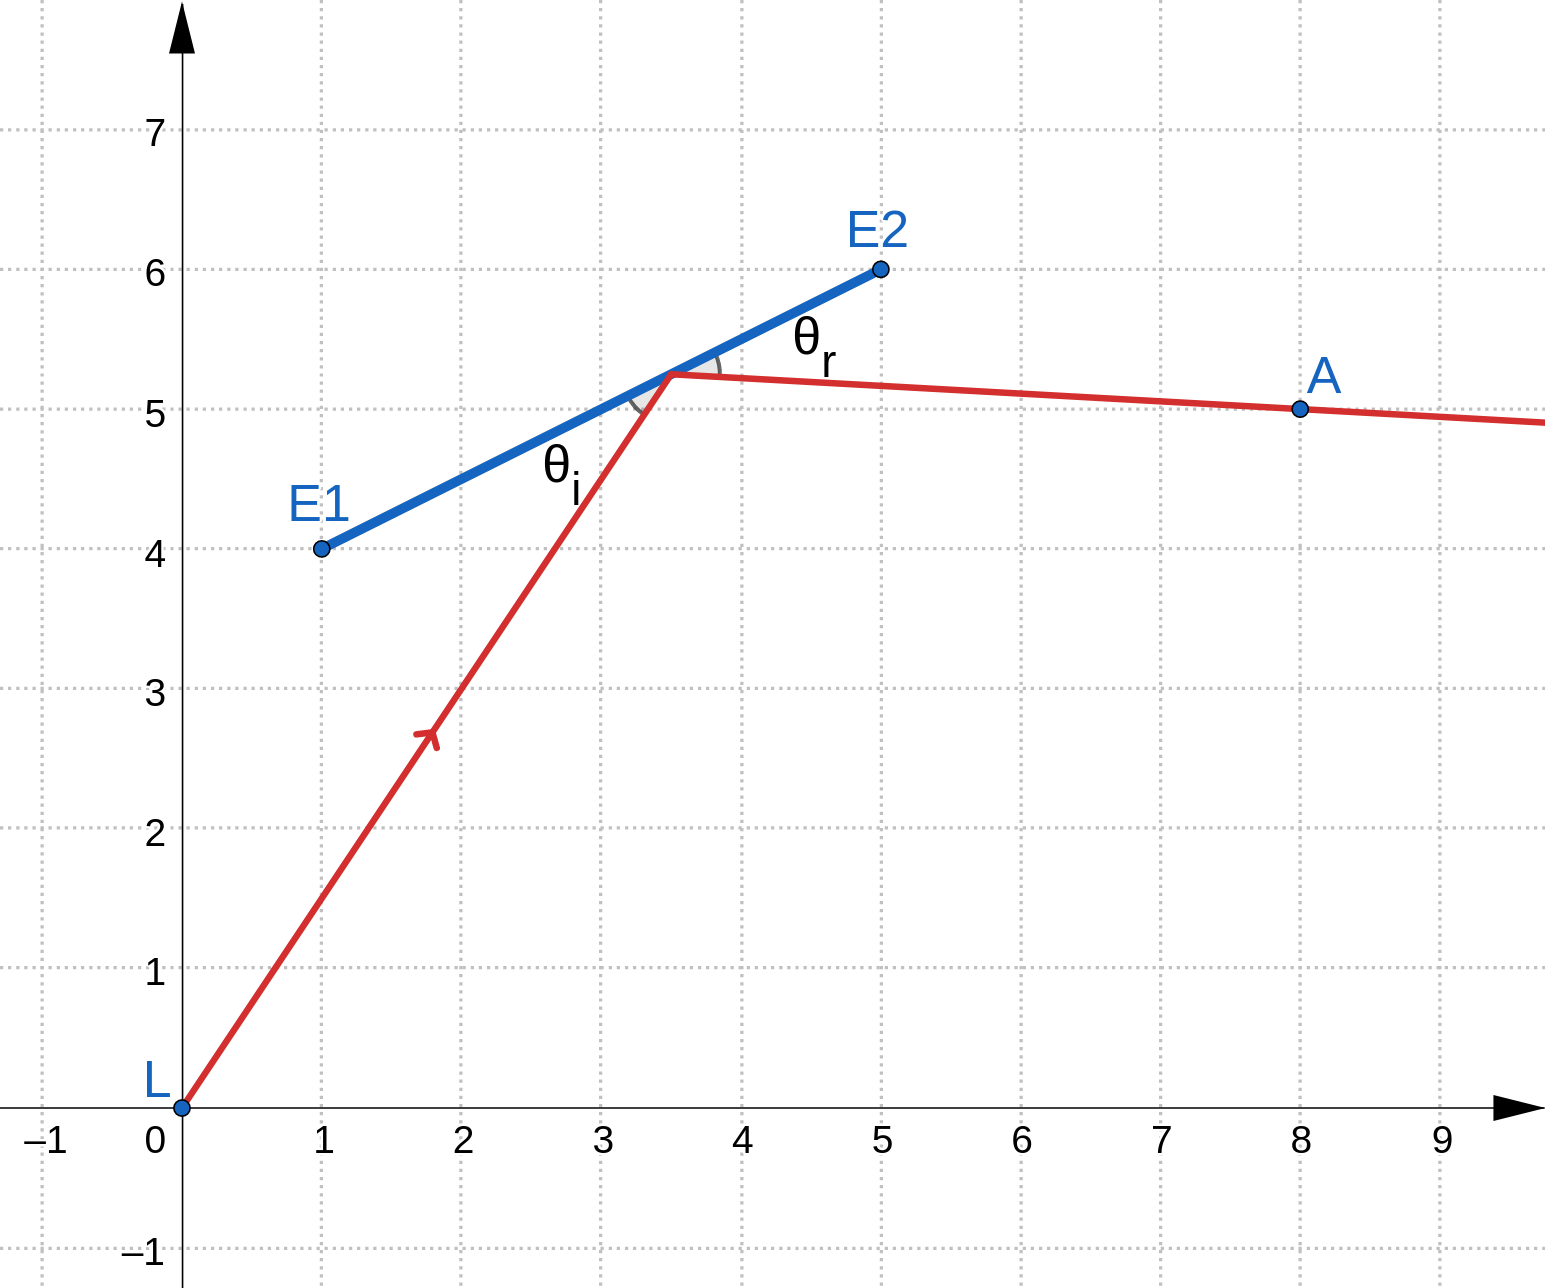
\includegraphics[width=12.0cm, height=9.5cm]{Teste1.png}

Imagem do primeiro caso de teste.
\end{center}

Leonardo é estudioso e sabe que o espelho em questão respeita as leis da física, ou seja, o ângulo de incidência é sempre igual ao ângulo de reflexão ($\theta_i = \theta_r$).

O espelho divide o plano em dois semi-planos. É garantido que Leonardo e Alberto estão localizados no mesmo semi-plano e que nenhum dos dois está em posição colinear com o espelho, e é possível desconsiderar Alberto e Leonardo como obstáculos, ou seja, o laser simplesmente os atravessa.

Ajude Leonardo a saber se é possível atingir Alberto com o laser através do espelho.